% Pgfplots demo
% Author: Christian Feuersänger
% Source: Pgfplots manual:
% http://www.ctan.org/tex-archive/help/Catalogue/entries/pgfplots.html
\documentclass{article}

\usepackage{tikz}
\usetikzlibrary{arrows,snakes,backgrounds}
\usepackage{pgfplots}
\pgfrealjobname{survey}
\begin{document}

\beginpgfgraphicnamed{graph1}
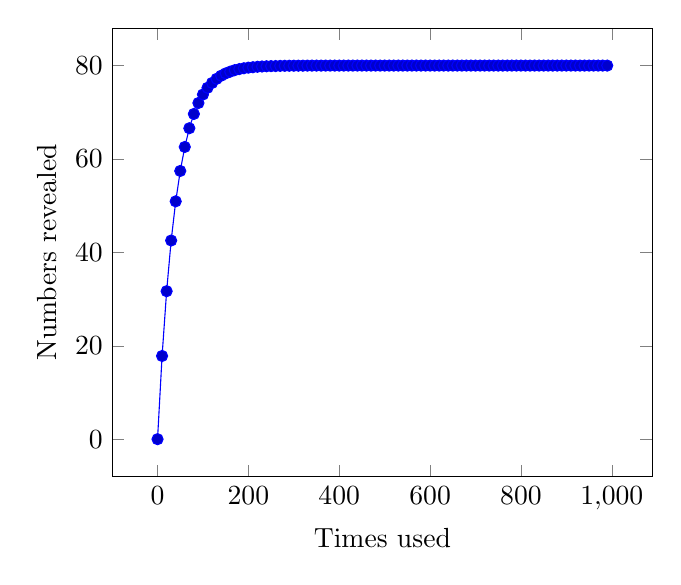
\begin{tikzpicture}
  \begin{axis}[
  xlabel=Times used,
  ylabel=Numbers revealed
  ]
  \addplot plot coordinates {
  (0, 0.0)
(10, 17.8166)
(20, 31.6906)
(30, 42.5432)
(40, 50.931)
(50, 57.4386)
(60, 62.5762)
(70, 66.5854)
(80, 69.6446)
(90, 71.9888)
(100, 73.8062)
(110, 75.2442)
(120, 76.2822)
(130, 77.1612)
(140, 77.8264)
(150, 78.3298)
(160, 78.7012)
(170, 79.0264)
(180, 79.2466)
(190, 79.4314)
(200, 79.5574)
(210, 79.6496)
(220, 79.743)
(230, 79.8064)
(240, 79.8534)
(250, 79.8866)
(260, 79.9048)
(270, 79.9362)
(280, 79.9514)
(290, 79.9634)
(300, 79.97)
(310, 79.9796)
(320, 79.9806)
(330, 79.9888)
(340, 79.9928)
(350, 79.992)
(360, 79.9936)
(370, 79.9958)
(380, 79.9964)
(390, 79.9976)
(400, 79.999)
(410, 79.9984)
(420, 79.999)
(430, 79.9988)
(440, 79.9996)
(450, 79.9998)
(460, 80.0)
(470, 79.9998)
(480, 79.9998)
(490, 80.0)
(500, 79.9996)
(510, 80.0)
(520, 80.0)
(530, 80.0)
(540, 80.0)
(550, 80.0)
(560, 80.0)
(570, 80.0)
(580, 80.0)
(590, 80.0)
(600, 80.0)
(610, 80.0)
(620, 80.0)
(630, 80.0)
(640, 80.0)
(650, 80.0)
(660, 80.0)
(670, 80.0)
(680, 80.0)
(690, 80.0)
(700, 80.0)
(710, 80.0)
(720, 80.0)
(730, 80.0)
(740, 80.0)
(750, 80.0)
(760, 80.0)
(770, 80.0)
(780, 80.0)
(790, 80.0)
(800, 80.0)
(810, 80.0)
(820, 80.0)
(830, 80.0)
(840, 80.0)
(850, 80.0)
(860, 80.0)
(870, 80.0)
(880, 80.0)
(890, 80.0)
(900, 80.0)
(910, 80.0)
(920, 80.0)
(930, 80.0)
(940, 80.0)
(950, 80.0)
(960, 80.0)
(970, 80.0)
(980, 80.0)
(990, 80.0)

};
  \end{axis}
\end{tikzpicture}

\endpgfgraphicnamed

\beginpgfgraphicnamed{graph2}
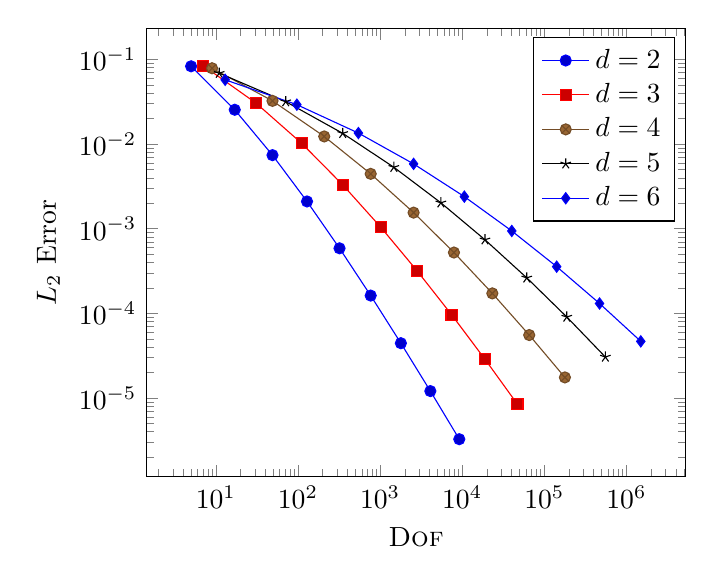
\begin{tikzpicture}
    \begin{loglogaxis}[
        xlabel=\textsc{Dof},
        ylabel=$L_2$ Error
    ]
    \axispath\draw
            (7.49165,-10.02171)
        |-  (8.31801,-11.32467)
        node[near start,left] {$\frac{dy}{dx} = -1.58$};
      \addplot plot coordinates {
        (5,     8.312e-02)
        (17,    2.547e-02)
        (49,    7.407e-03)
        (129,   2.102e-03)
        (321,   5.874e-04)
        (769,   1.623e-04)
        (1793,  4.442e-05)
        (4097,  1.207e-05)
        (9217,  3.261e-06)
    };

    \addplot plot coordinates {
        (7,     8.472e-02)
        (31,    3.044e-02)
        (111,   1.022e-02)
        (351,   3.303e-03)
        (1023,  1.039e-03)
        (2815,  3.196e-04)
        (7423,  9.658e-05)
        (18943, 2.873e-05)
        (47103, 8.437e-06)
    };

    \addplot plot coordinates {
        (9, 7.881e-02)
        (49,    3.243e-02)
        (209,   1.232e-02)
        (769,   4.454e-03)
        (2561,  1.551e-03)
        (7937,  5.236e-04)
        (23297, 1.723e-04)
        (65537, 5.545e-05)
        (178177,    1.751e-05)
    };

    \addplot plot coordinates {
        (11,    6.887e-02)
        (71,    3.177e-02)
        (351,   1.341e-02)
        (1471,  5.334e-03)
        (5503,  2.027e-03)
        (18943, 7.415e-04)
        (61183, 2.628e-04)
        (187903,    9.063e-05)
        (553983,    3.053e-05)
    };

    \addplot plot coordinates {
        (13,    5.755e-02)
        (97,    2.925e-02)
        (545,   1.351e-02)
        (2561,  5.842e-03)
        (10625, 2.397e-03)
        (40193, 9.414e-04)
        (141569,    3.564e-04)
        (471041,    1.308e-04)
        (1496065,   4.670e-05)
    };
    \legend{$d=2$\\$d=3$\\$d=4$\\$d=5$\\$d=6$\\}

    \end{loglogaxis}
\end{tikzpicture}
\endpgfgraphicnamed
\end{document}
